\subsubsection{Adaptive Naive Bayes Classifier (ANBC)} \label{sec:anbc} ANBC \cite{14} is a supervised learning algorithm that can be used to classify any type of N-dimensional signal. It is based on simple probabilistic classifier called Naive Bayes classifier. It fundamentally works by fitting an N-dimensional Gaussian distribution to each class during the training phase. New gestures can then be recognized in the prediction phase by finding the gesture that results.

ANBC like Naive Bayes classifier makes a number of basic assumptions with input data that all the variables in the data are independent. However, despite these naive assumptions, Naive Bayes Classifiers have proved successful in many real-world classification problems \cite{15}. It has also been shown in a study that the Naive Bayes Classifier not only performs well with completely independent features, but also with functionally dependent features.

ANBC algorithm is based on Bayes theory and gives the likelihood of event $A$ occurring, given the observation of event $B$. In the equation \ref{eq:grt:bayes}, $P(A)$ represents the prior probability of event $A$ occurring and $P(B)$ is a normalizing factor to ensure that all the posterior probabilities sum to 1.

\begin{equation}
P(A|B) = \frac{P(B|A) P(A)}{P(B)}
\label{eq:grt:bayes}
\end{equation}

\paragraph*{Training} The weighting coefficient adds an important feature for the ANBC algorithm as it enables one general classifier to be trained with multi-dimensional inputs, even if a number of inputs are only relevant for one particular gesture. For example, if it is used to recognize hand gestures, the weighting coefficients would enable the classifier to recognize both left and right hand gestures independently, without the position of the left hand affecting the classification of a right handed gesture. In this case left hand gestures will have weights {1,1,1,0,0,0}, right hand gestures will have weights {0,0,0,1,1,1} and both hand gestures will have weights {1,1,1,1,1,1}.

Using the weighted Gaussian model, the ANBC algorithm requires $G(3N)$ parameters, assuming that each of the $G$ gestures require specific values for the N-dimensional $ \mu_{k} , \sigma_{k}^{2} $ and $ \phi_{k} $ vectors where $ \mu_{k} , \sigma_{k}^{2},\phi_{k}$ are mean, variance and weighting coefficients. Assuming that $ \phi_{k} $ is set by the user, $ \mu_{k} $ and $\sigma_{k}^{2} $ values can easily be calculated in a supervised learning scenario by grouping the input training data $X$ into a matrix containing $M$ training examples each with $N$ dimensions, into their corresponding classes. The values for $ \mu$ and $\sigma^{2} $of each dimension $n$ for each class $k$ can then be estimated by computing the mean and variance of the grouped training data for each of the respective classes \cite{14}.

\begin{equation}
P(g_{k}|x) = \frac{P(x|g_{k}) P(g_{k})} {\sum_{i=1}^{G}P(x|g_{i}) P(g_{i})} \:\:\:\:\: 1\leq k \leq G
\label{eq:grt:gauss}
\end{equation}

After the Gaussian models have been trained for each of the $G$ classes, an unknown N-dimensional vector $x$ can be classified as one of the $G$ classes using the maximum a posterior probability estimate (MAP). MAP estimate classifies $x$ as the $k$-th class that results in the maximum a posterior probability given by the equation \ref{eq:grt:gauss}

\begin{equation}
ln N (x|\Phi_{k}) \:\:\:\:\: 1\leq k \leq G
\label{eq:grt:threshold}
\end{equation}

\paragraph*{Rejection Threshold} Using equation \ref{eq:grt:threshold}, an unknown N-dimensional vector $x$ can be classified as one of the $G$ classes from a trained ANBC model. If $x$ actually comes from an unknown distribution that has not been modeled by one of the trained classes then, it will be incorrectly classified against the $k$ th gesture that gives the maximum likelihood value. A rejection threshold must therefore be calculated for each of the $G$ gestures to enable the algorithm to classify any of the $G$ gestures from a continuous stream of data that also contains non-gestural data \cite{14}.

\paragraph*{Online Training} One key element of ANBC is that it can easily be made adaptive. Adding an adaptive online training phase to the common two-phase (training and prediction) provides some significant advantages for the recognition gestures. During online training phase the algorithm will not only perform real-time predictions on the continuous stream of input data, but it will also continue to train and refine the models for each gesture. This enables the user to initially train the algorithm with a low number of training samples and during the adaptive online training phase, the algorithm can continue to train and refine the initial models, creating a more robust model as the number of training samples increases.

\paragraph*{Pros / Cons} ANBC works well for the classification of static gestures and non-temporal pattern recognition. However, the main limitation of the ANBC is that, it does not work well when the data you want to classify, is not linearly separable because it uses a Gaussian distribution to represent each class. Also when ANBC is working with online training enabled, a small number of incorrectly labeled training examples could create a loose model that becomes less effective at each update step and ultimately lead to a poor performance and accuracy.

\subsubsection{Gesture Recognition Toolkit (GRT)} \label{sec:grt} Gesture Recognition Toolkit is a cross-platform open-source C++ library designed and developed mainly by Nicholas Gillian at MIT Media Lab to make real-time machine learning and gesture recognitions \cite{16}. Emphasis is placed on the ease of use with a consistent, minimalist design that promotes accessibility while supporting flexibility and customization for advanced users. The toolkit features a broad range of classification and regression algorithms, and has extensive support for building real-time systems. GRT includes algorithms for signal processing, feature extraction and automatic gesture spotting. 

In this thesis, we attempt to take advantage of GRT as framework to carry out most of the tasks involved in hand gesture recognition. Figure \ref{fg:grt:pipeline} shows that GRT provides the full fledge pipeline to build a real-time gesture recognition system. 

\begin{figure}
	[h] \hspace{-5 mm} 
	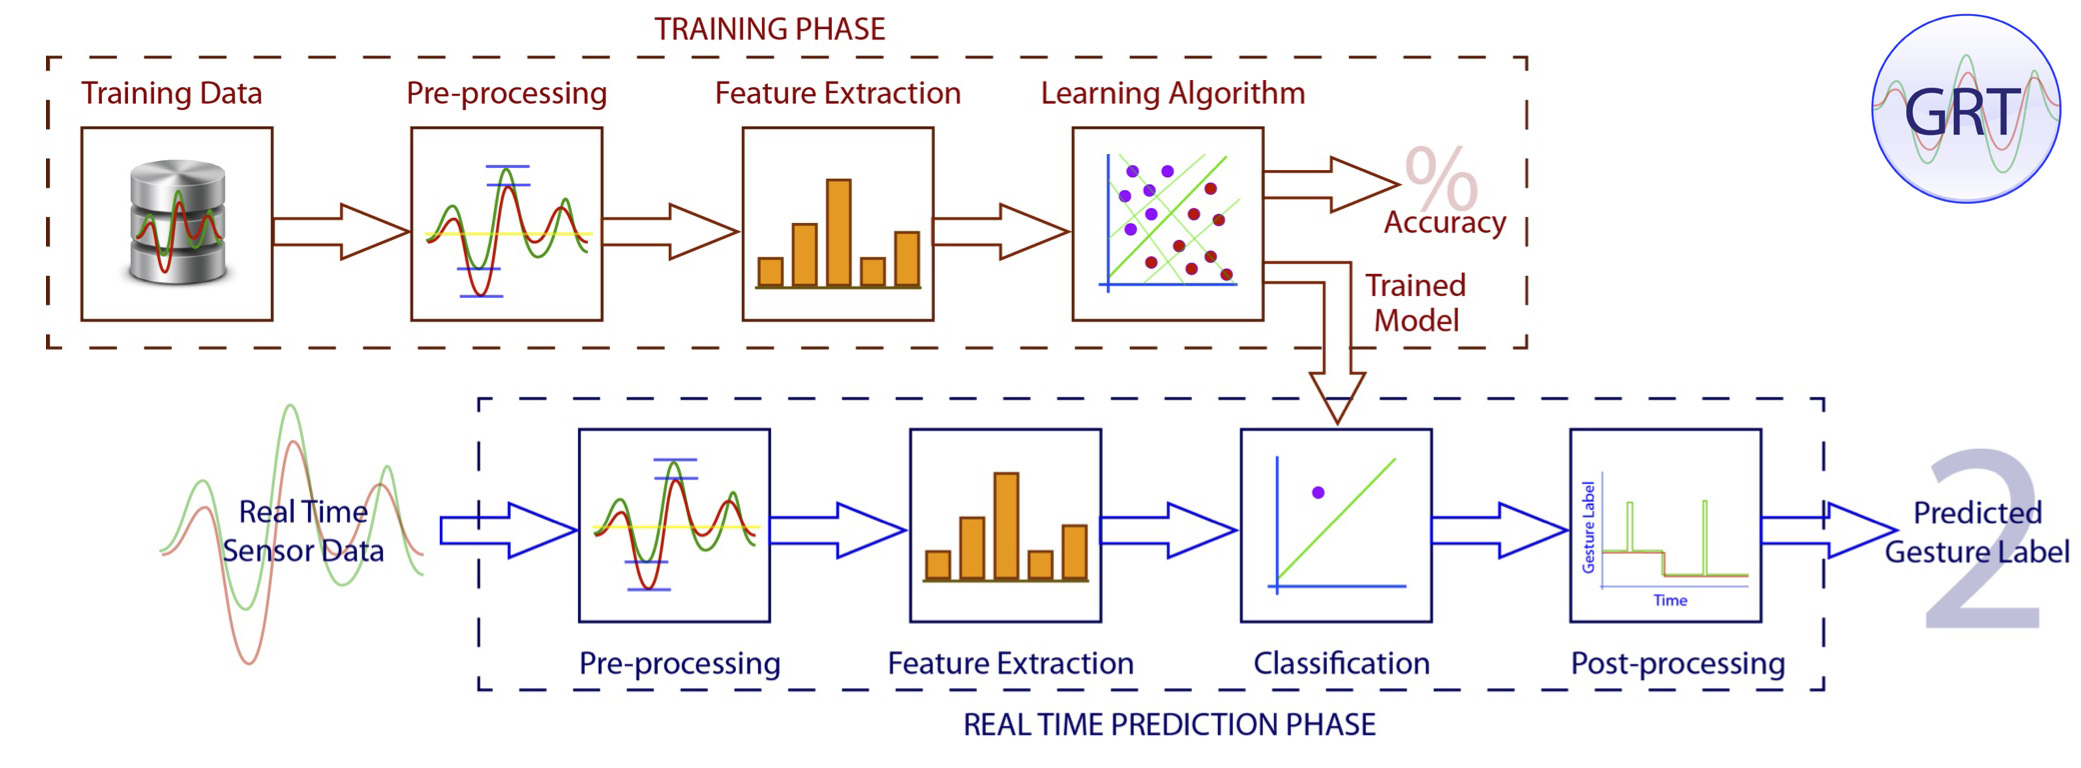
\includegraphics[width=160mm]{figures/content/grt-pipeline.jpg} \caption{Stages of Gesture Recognition which are supported by GRT Recognition Pipeline. \cite{16} } \label{fg:grt:pipeline} 
\end{figure}


\paragraph*{Pipeline} GRT provides an API to reduce the need for boilerplate code to perform common functionality, such as passing data between algorithms or to per-process data sets. GRT uses an object-oriented modular architecture and it is built around a set of core modules and a gesture-recognition pipeline. The input to both the modules and pipeline consists of an N-dimensional double-precision vector, making the toolkit flexible to any type of input signal. The algorithms can be used as stand-alone classes; alternatively a gesture recognition pipeline can be used to chain modules together to create a more sophisticated gesture-recognition system. Modularity of GRT pipeline offers developers opportunities to work on each stages of gesture recognition independently. Additionally pipeline can be stored and loaded dynamically so that an compiled application can work in many different configurations. 

\paragraph*{ClassificationData} Accurate labeling of dataset is very critical for machine learning problems. The toolkit thus contains an extensive support for recording, labeling and managing supervised and unsupervised datasets for classification, regression and time series analysis. \textit{ClassificationData} is the data structure used for supervised learning problems and for most of the non-temporal classification algorithms.

GRT allows us to store and load the training data in GRT format or Comma Separated Values (CSV). Since the training datasets are stored in human readable format, it enables us to add more samples which are collected separately or remove false data from the training dataset.

\paragraph*{TrainingDataRecordingTimer} Important part of the training phase is recording positive samples of modeled hand gestures. Hence, GRT provides a feature called \textit{TrainingDataRecordingTimer} that sets recording and preparation time in milliseconds. Once it is started by calling \textit{startRecording(prepationTime, recordTime)} method, it waits for given preparation time before it actually starts to store the data. This feature helps the trainer get into the right pose before samples are added to the training data and as well as train all the gestures for the same time duration.

\paragraph*{Algorithms} GRT features a broad range of machine-learning algorithms such as AdaBoost, Decision Trees, Dynamic Time Warping (DTW), Hidden Markov Models (HMM), K-Nearest Neighbor (KNN), Linear and Logistic Regression, Adaptive Naive Bayes (ANBC), Multilayer Perceptrons (MLP), Random Forests and Support Vector Machines (SVM) \cite{16}. 

\paragraph*{Null Rejection} Another important feature of GRT is Null Rejections threshold. It means that algorithms can automatically spot the difference between trained gestures and unintended gestures that can happen when the user moves the hand in freely. It can be enabled by the method \textit{enableNullRejection(true)} and the range of the null rejection region can be set by this method \textit{setNullRejectionCoeff(double nullRejectionCoeff)} of the classifier. Algorithm such as the ANBC and N-Dimensional DTW, learn rejection thresholds from the training data, which are then used to automatically recognize valid gestures from a continuous stream of real-time data.

\begin{figure}
	[h] \centering 
	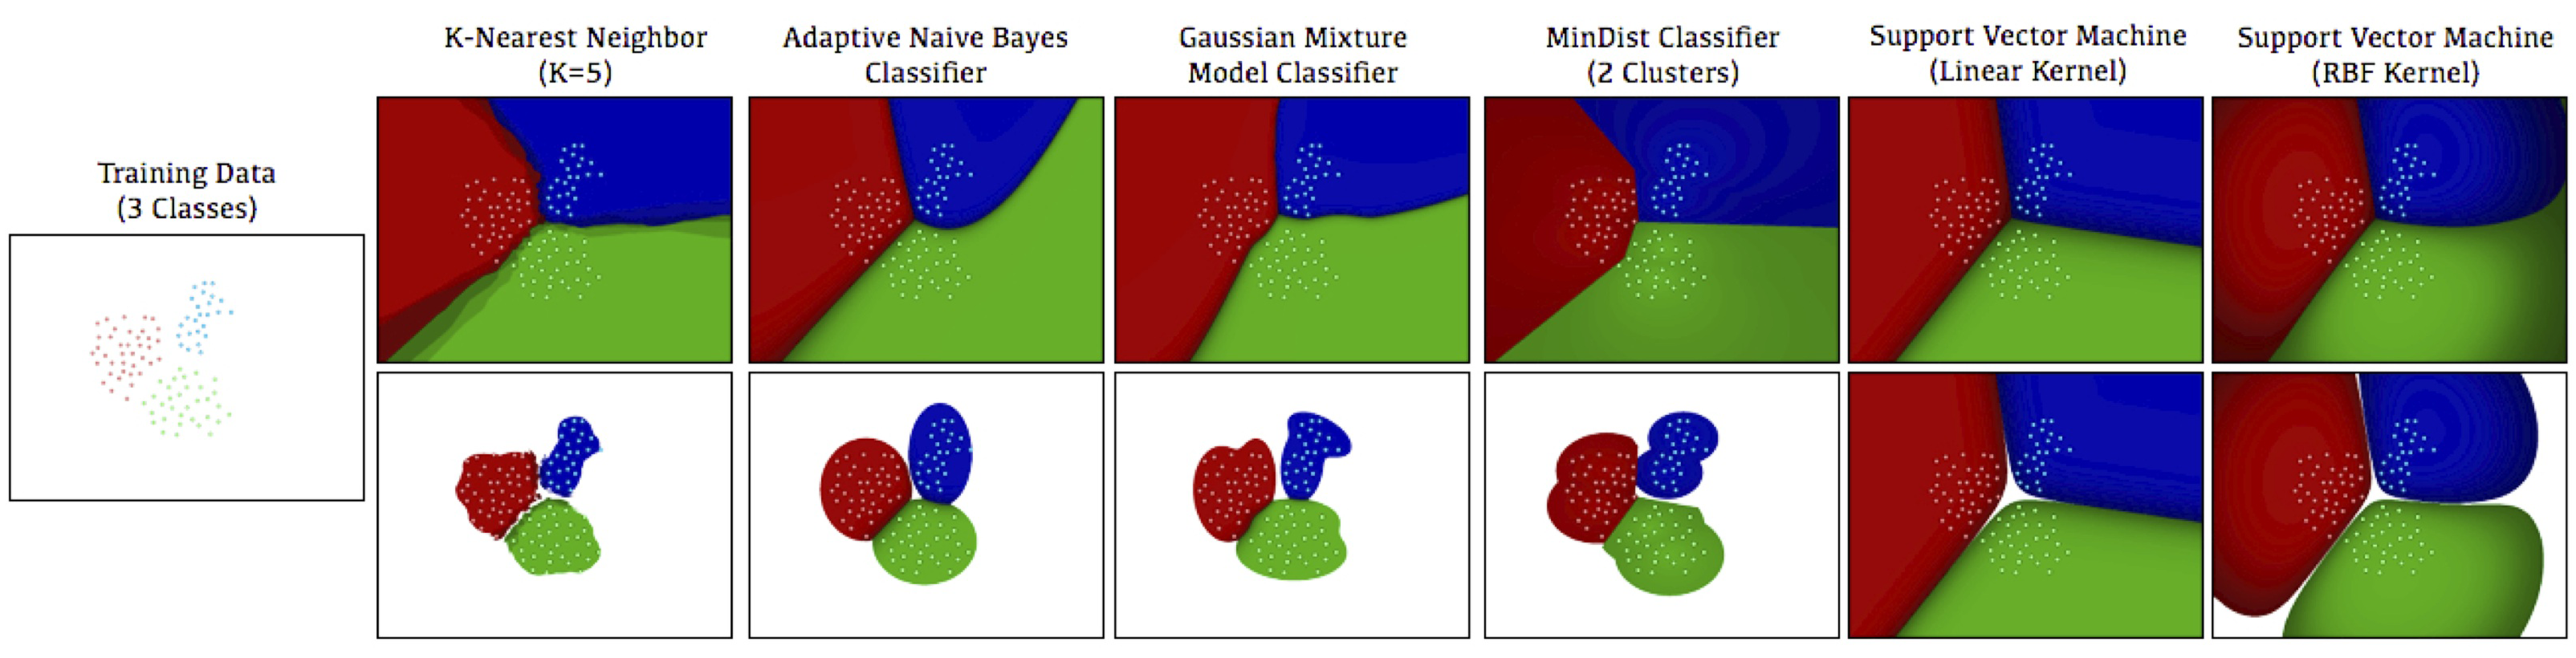
\includegraphics[height=35mm]{figures/content/grt-null.png} \caption{GRT Null Rejection} \label{fg:grt:null} 
\end{figure}


Figure \ref{fg:grt:null} shows that the decision boundaries computed by training six of classification algorithms on an example dataset with 3 classes. After training each classifier, each point in the two-dimensional feature space is colored by the likelihood of the predicted class label (red for class 1, green for class 2, blue for class 3). The top row shows the predictions of each classifier with null rejection disabled. The bottom row shows the predictions of each classifier with null rejection enabled with a coefficient of 3.0. Rejected points are colored white. Note that both the decision boundaries and null-rejection regions are different for each of the classifiers. This results from the several learning and prediction algorithms used by each classifier. 

\paragraph*{Scaling Normalization} Real-time classification faces normalization problems when the range of training data differ from prediction input. To solve this problems, there are few solutions such as Z-score Standardization and Feature Scaling. GRT presents a simple solution called as Minimum-Maximum scaling.

Min-Max scaling rescales the range in [0, 1] or [-1, 1]. Selecting the target range depends on the nature of the data. Classifiers \textit{enableScaling(true)} method scales input vector between the default min-max range that is from 0 to 1. The cost of having this bounded range is that model will end up with smaller standard deviations, which can suppress the effect of outliers. Equation \ref{eq:grt:scaling} shows how Min-Max scaling is done.

\begin{equation}
\large 
x{}' = \frac{x - min(x)}{max(x) - min(x)}
\label{eq:grt:scaling}
\end{equation}

\paragraph*{Pre/Post Processing Modules} In many real-world scenarios, the input to a classification algorithm must be preprocessed and have salient features extracted. GRT therefore supports a wide range of pre/post-processing modules such as Moving Average Filter, Class Label Filter and Class Label Change Filter, embedded feature extraction algorithms such as AdaBoost, dimensionality reduction techniques such as Principal Component Analysis (PCA) and unsupervised quantizers such as K-Means Quantizer, Self-Organizing Map Quantizer.

There will not be any need of preprocessing modules in this project since raw data received from depth sensor is processed by NiTE framework. However, post-processing modules such as Class Label Filter and Class Label Change Filter may be needed for a reasons that depth sensor samples 30 frames per second, therefore 30 input samples per second are supplied to the classifier for prediction and the output must be triggered once for every gesture. 

\begin{figure}
	[h] \centering 
	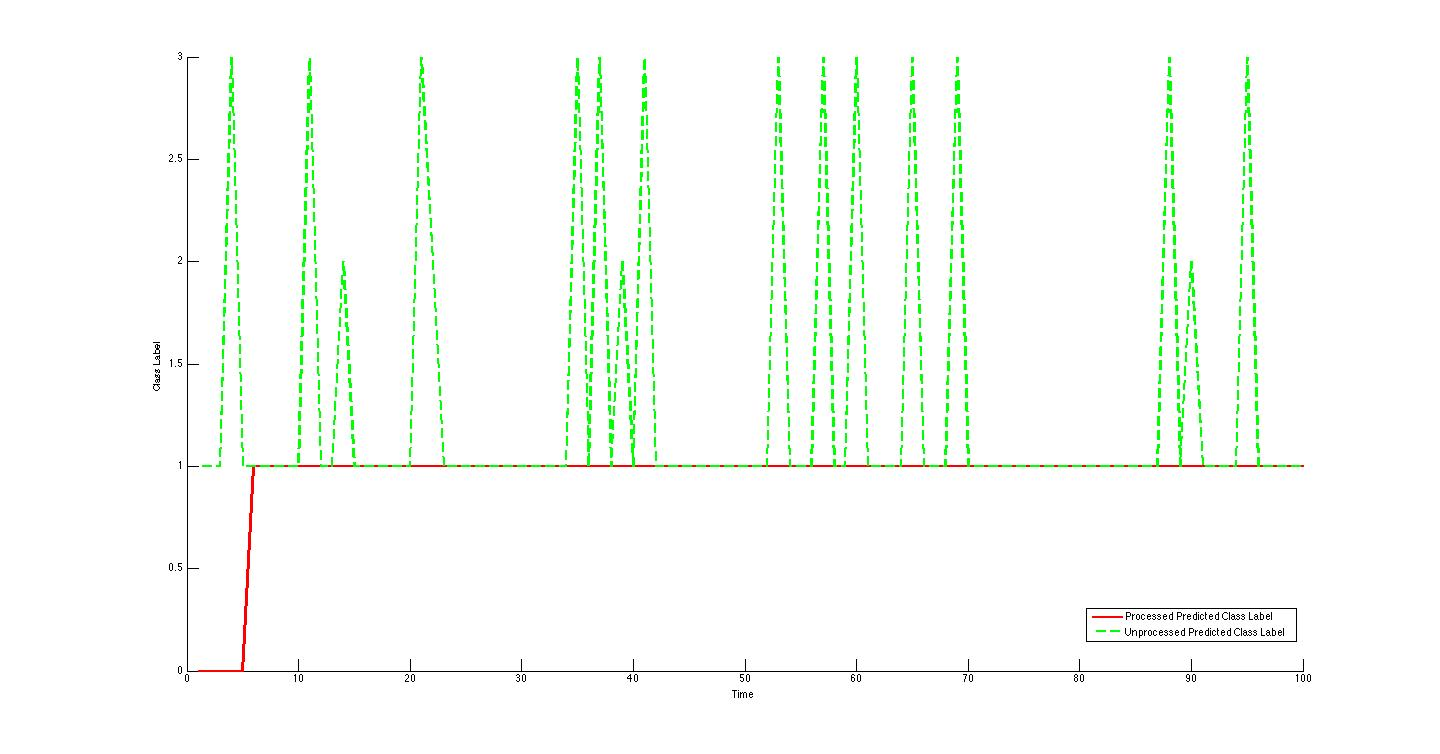
\includegraphics[height=7cm]{/content/grt-label-filter.jpg} \caption{GRT Class Label Filter removes the sporadic prediction values and outputs buffered class label. \cite{16}} \label{fg:grt:label} 
\end{figure}


\paragraph*{Class Label Filter} It is a useful post-processing module which can remove erroneous or sporadic prediction spikes that may be made by a classifier on a continuous input stream of data. Figure \ref{fg:grt:label} that the classifier correctly outputs the predicted class label of 1 for a large majority of the time that a user is performing gesture 1. However, may be due to sensor noise or false samples in the training data, the classifier outputs the class label of 2. In this instance the class label filter can be used to remove these sporadic prediction values with the output of the class label filter in this instance being 1. 

Class Label Filter module is controlled through two parameters: the minimum count value and buffer size value. The minimum count sets the minimum number of label values that must be present in the buffer to be output by the Class Label Filter. The size of the class labels buffer is set by the buffer size parameter. If there is more than one type of class label in the buffer then the class label with the maximum number of instances will be output. If the maximum number of instances for any class label in the buffer is less than the minimum count parameter then the Class Label Filter will output the default null rejection class label of 0.

\begin{figure}
	[h] \centering 
	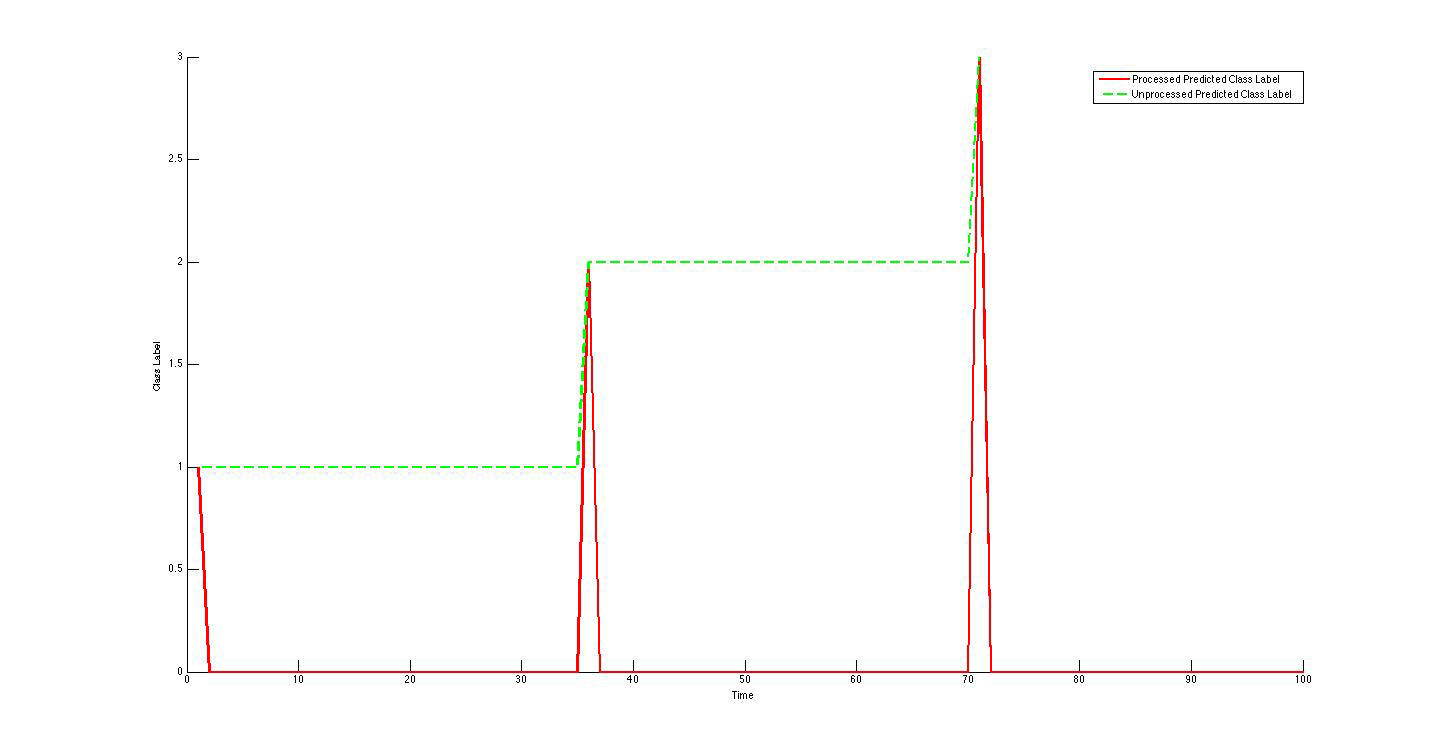
\includegraphics[height=7cm]{figures/content/grt-label-change-filter.jpg} \caption{GRT Label Change Filter outputs only when there is change in the prediction. \cite{16}} \label{fg:grt:label:change} 
\end{figure}


\paragraph*{Class Label Change Filter} It is one of the useful post-processing module that triggers when the predicted output of a classifier changes. Figure \ref{fg:grt:label:change}shows that, if the output stream of a classifier is {1,1,1,1,2,2,2,2,3,3}, then the output of the filter would be {1,0,0,0,2,0,0,0,3,0}. This module is useful to trigger a gesture only once if the user is gesticulating the same gesture for longer time duration. 

\paragraph*{GUI} Figure \ref{fg:grt:gui} shows GRT-GUI which is an application that provides an easy-to-use graphical interface developed in C++ to setup and configure a gesture recognition pipeline that can be used for classification, regression, or time-series analysis. Data and control commands are streamed in and out of this application as Open Sound Control (OSC) packets via UDP . Therefore, it acts as a standalone application to record, label, save, load and test the training data and performs a real-time prediction for the incoming data, send output to another application. 

\begin{figure}
	[h] \centering 
	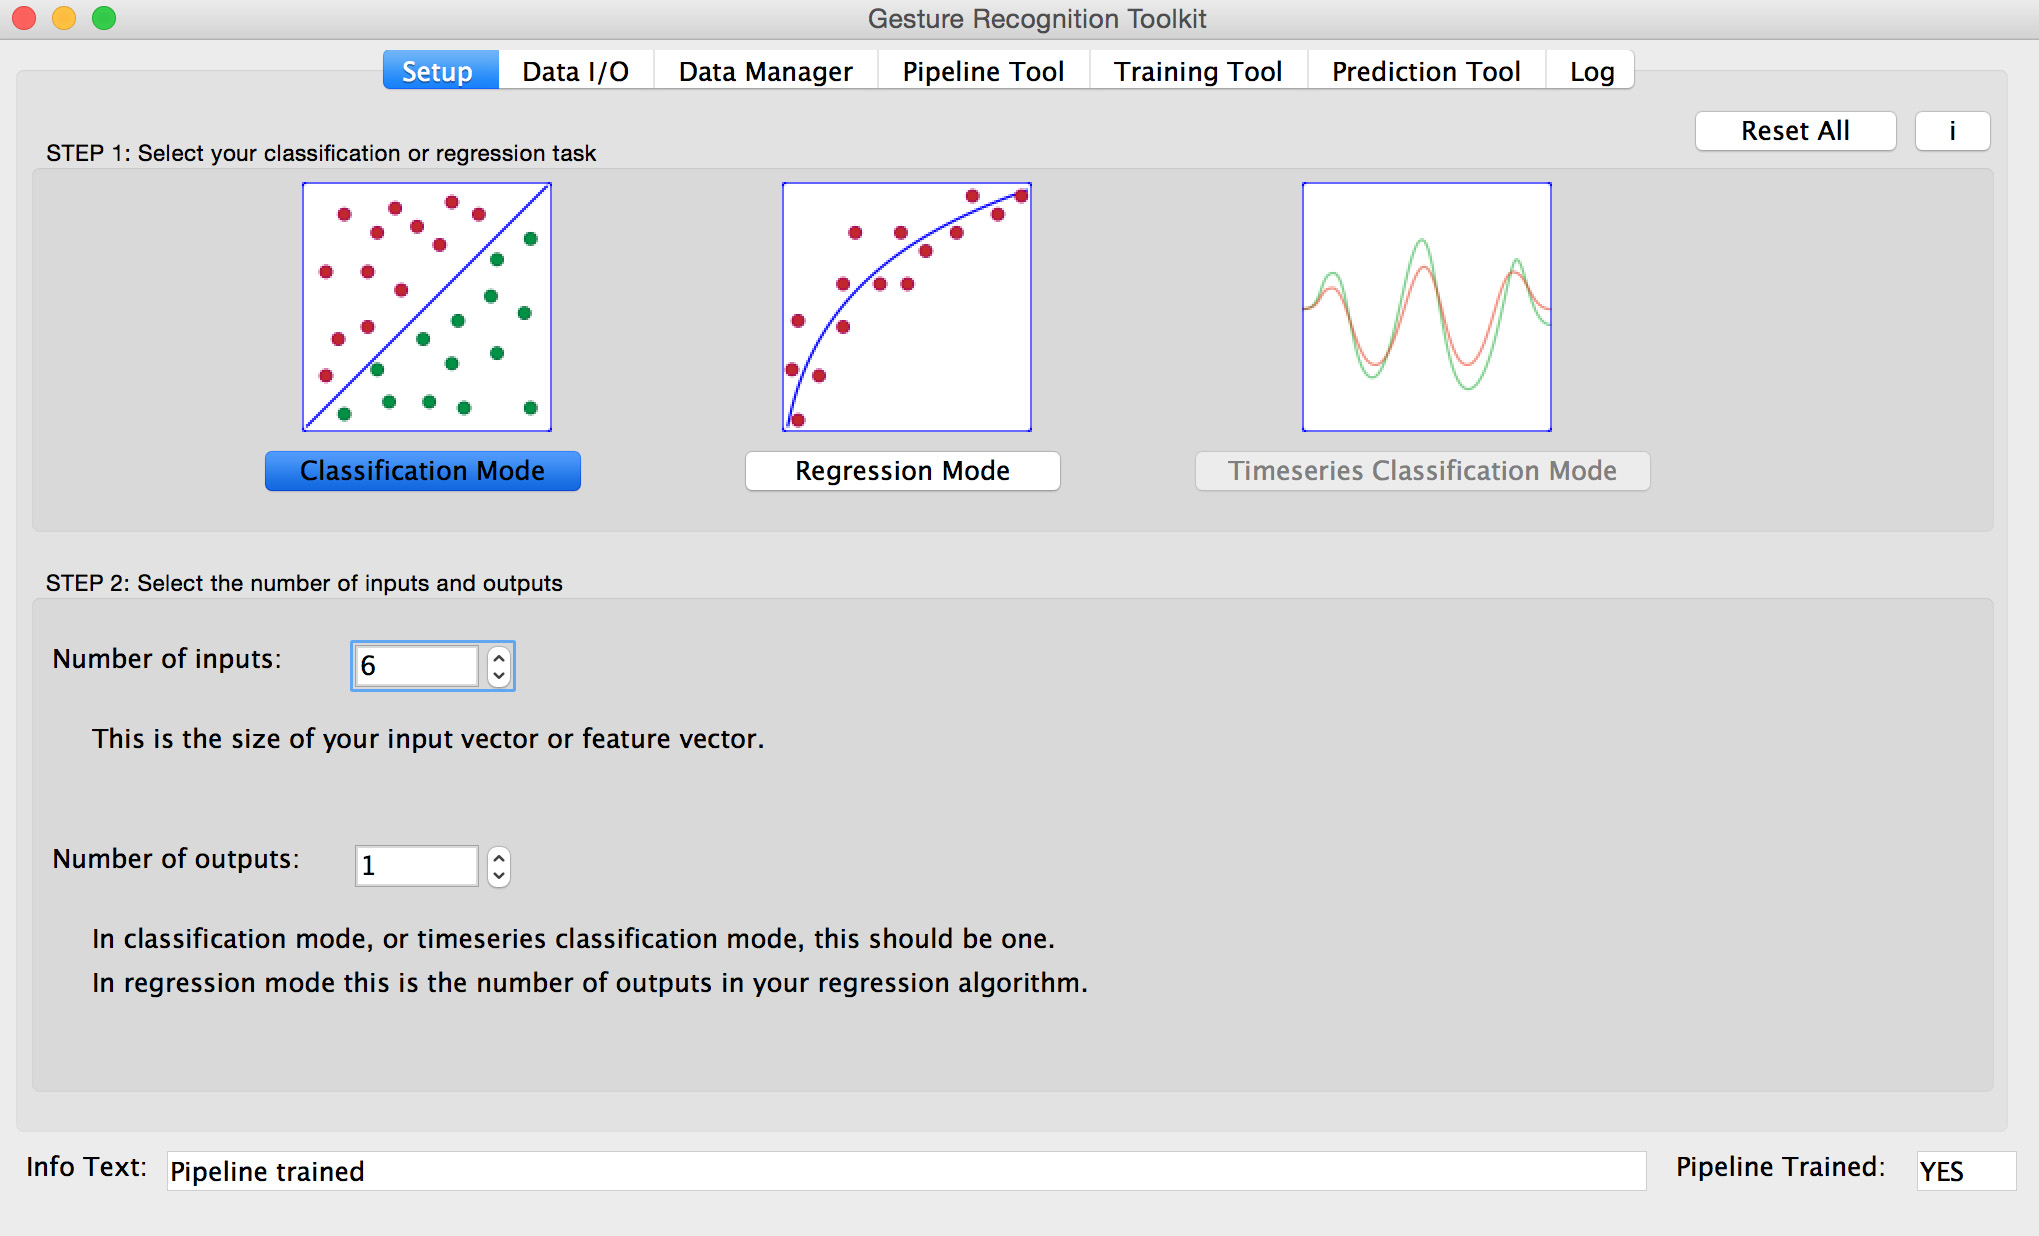
\includegraphics[height=7cm]{figures/content/grt-gui.jpg} \caption{GRT GUI is an standalone application to quick prototype by recording, labeling, saving, loading, testing the training data and to perform a real-time prediction. \cite{grt-spec}} \label{fg:grt:gui} 
\end{figure}
 
